\chapter{Z Tanım Bölgesinde Kök Eğrisi}
Z tanım bölgesinde bir transfer fonksiyonu $T=0.2$ olmak üzere
\begin{equation}
    G(z)=\frac{1}{z^3 + 0.4 z^2 - 0.37 z - 0.04}
\end{equation}
olarak verilmiştir. P kontrolör ile kapalı çevrim transfer fonksiyonu
\begin{equation}
\begin{split}
    T(z)&=\frac{kG(z)}{1+kG(z)}\\
    T(z)&=\frac{\frac{k}{z^3 + 0.4 z^2 - 0.37 z - 0.04}}{1+\frac{k}{z^3 + 0.4 z^2 - 0.37 z - 0.04}}\\
    T(z)&=\frac{k}{z^3 + 0.4 z^2 - 0.37 z - 0.04+k}
\end{split}
\end{equation}
olarak hesaplanır. 

\begin{figure}[!htb]
    \centering
    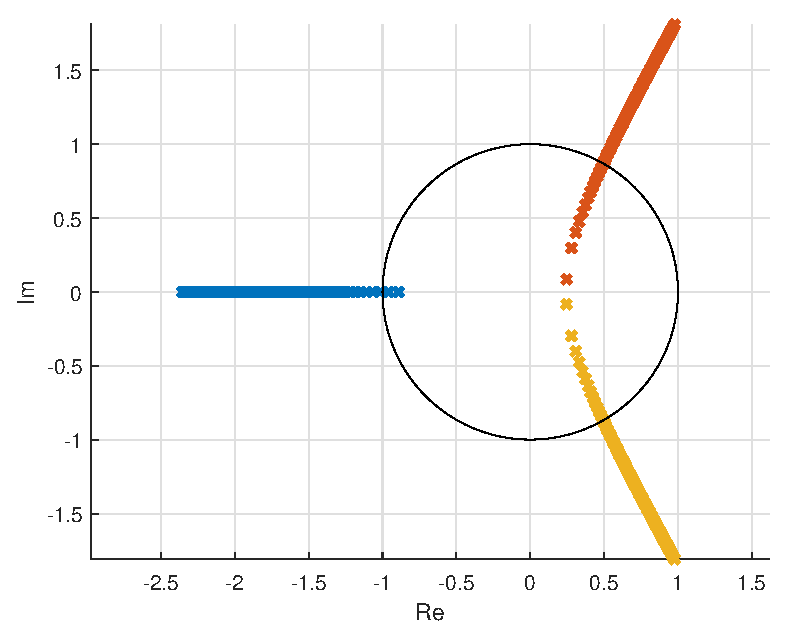
\includegraphics[width=0.75\textwidth]{img/lec5_rlocus1}
    \caption{Sisteme ait kök eğrisi}
    \label{fig:lec5_rlocus1}
\end{figure}

